\documentclass{book}
\usepackage{graphicx}
\usepackage[utf8]{inputenc}
\usepackage[paperheight=210mm, paperwidth=210mm, margin=2cm, heightrounded]{geometry}
\usepackage{calligra}
\usepackage[T1]{fontenc}
\usepackage{setspace}
\author{Rachel Hiskins}
\calligra
\title{{\Huge A quiet conversation within a mandala}\\[15pt]
\space
\texttt{An inquiry into the therapeutic \\benefits of creating a mindful mandala}}

\date {December 2016}
\makeindex
\begin{document}
\begin{titlepage}
	\calligra
    \maketitle
\end{titlepage}
\doublespacing 

\begin{description}
\item[ Submitted in partial fulfilment of the requirements for the degree of Masters of Therapeutic Arts by Supervision. The MIECAT Institute, Melbourne, Australia
Statement of Authorship] 
\end{description}
%Introduction (chapter)
	\chapter{Introduction}

\begin{figure}[htbp]
\begin{center}
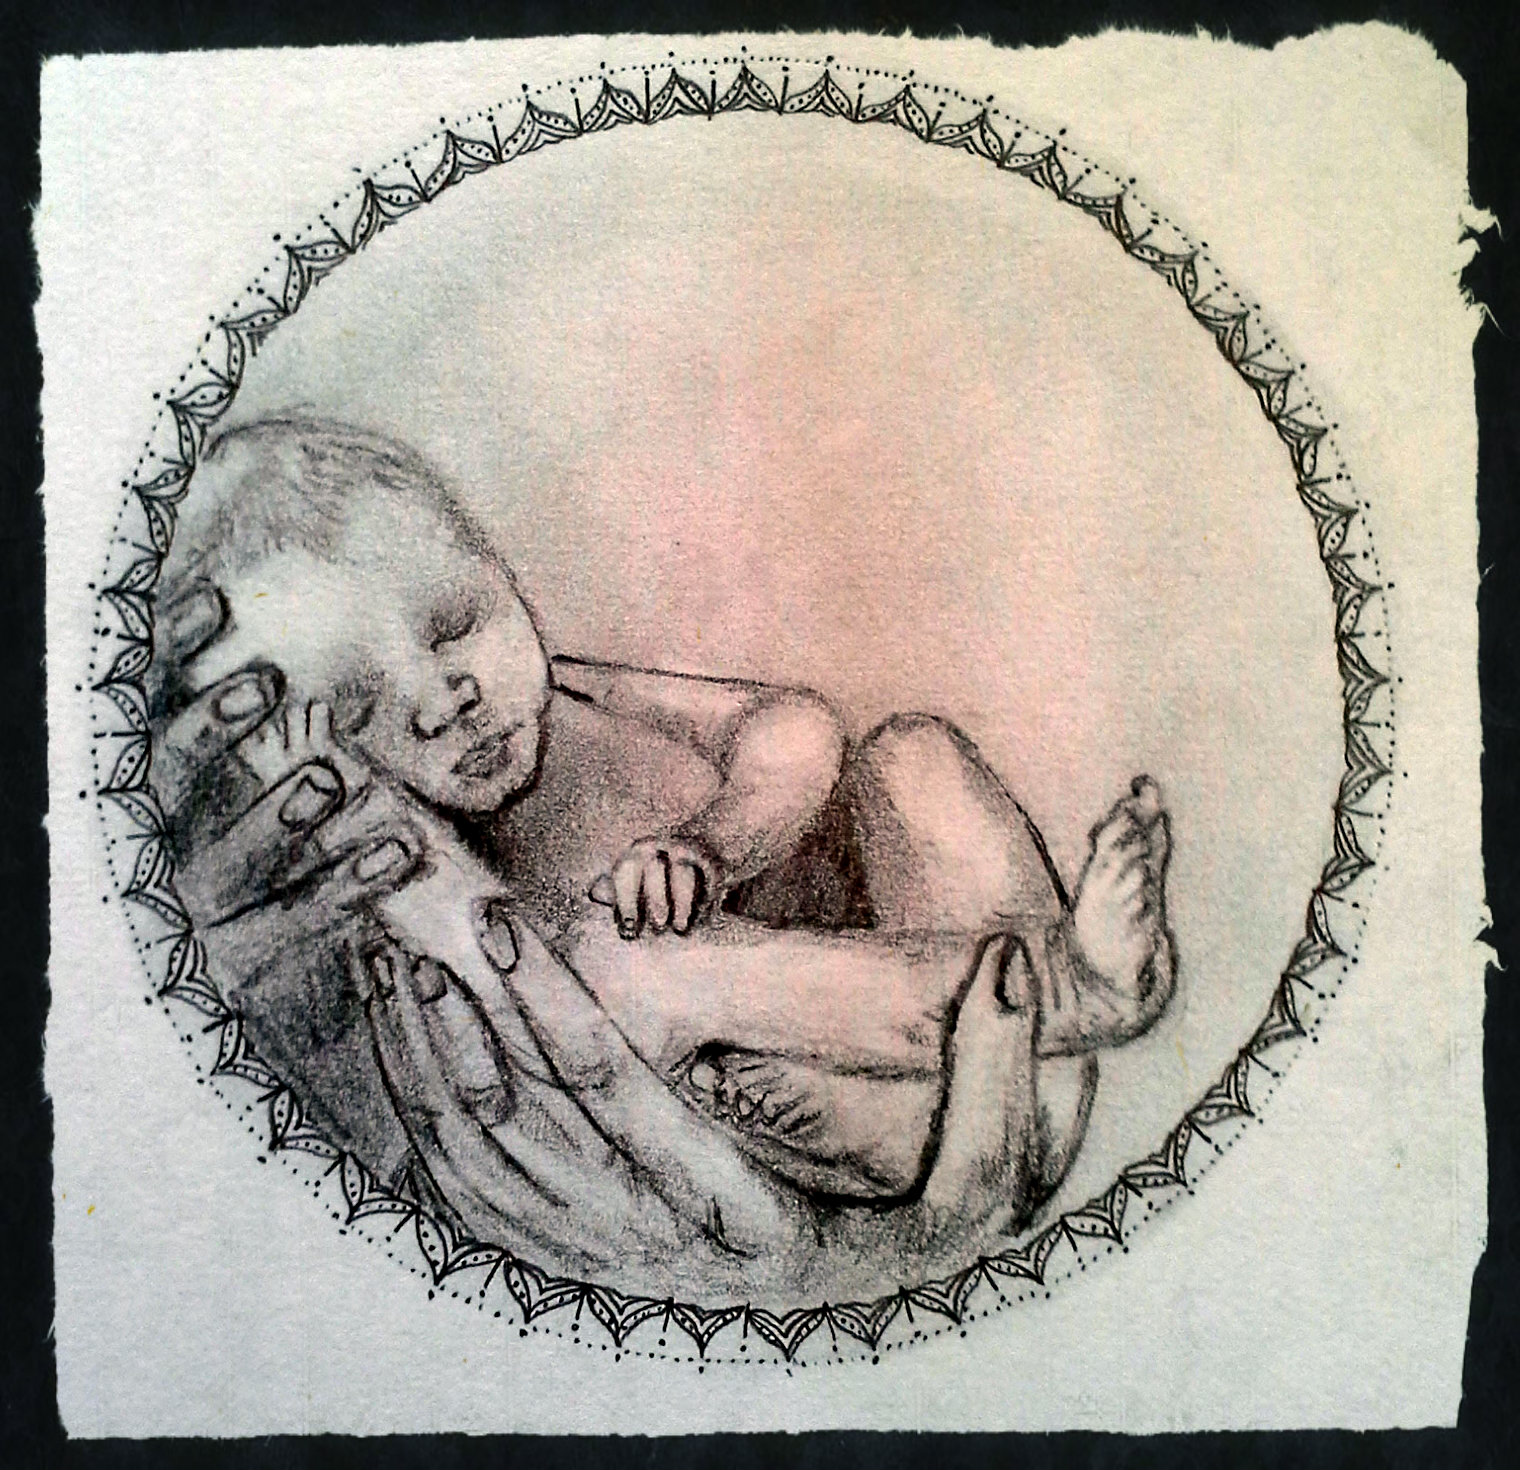
\includegraphics[scale=.25]{../eps/babymandala_1.eps} 
\caption{The birth of creating}
\label{label}
\end{center}
\end{figure}

%\begin{quote}
%"Let each man exercise the art he knows"
%\end{quote}

\newpage 


For many years mandalas have been a huge part of my life. I have been creating mandalas since 2003, when I was first introduced to the Jungian perspective on mandalas and the transpersonal approach. I have used mandalas in my private practice, provided workshops in Cambodia and have and will continue to use mandalas as a reflective tool. Consequently, all my experiences have led to my inquiry into conversations within mandalas.

I studied Fine Arts at the University of Maryland in the United States of America between 1998-2001 on a hockey scholarship and was highly influenced by abstract expressionism. As a result, I painted mainly expressionistic oil portraits and abstract paintings.


\begin{figure}[htbp]
\begin{center}
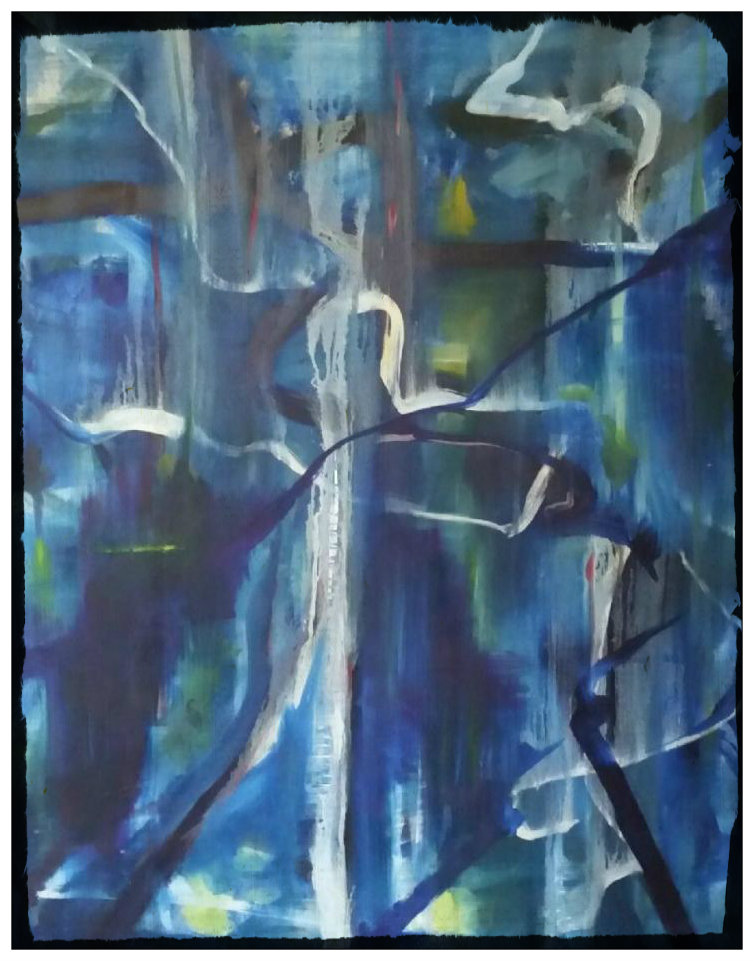
\includegraphics[scale=.25]{../eps/FIRST_ABSTRACT_PAINTING.eps}
\caption{FIRST ABSTRACT PAINTING, UNTITELED}
\label{label}
\end{center}
\end{figure}
\newpage 

\begin{figure}[htbp]
\begin{center}
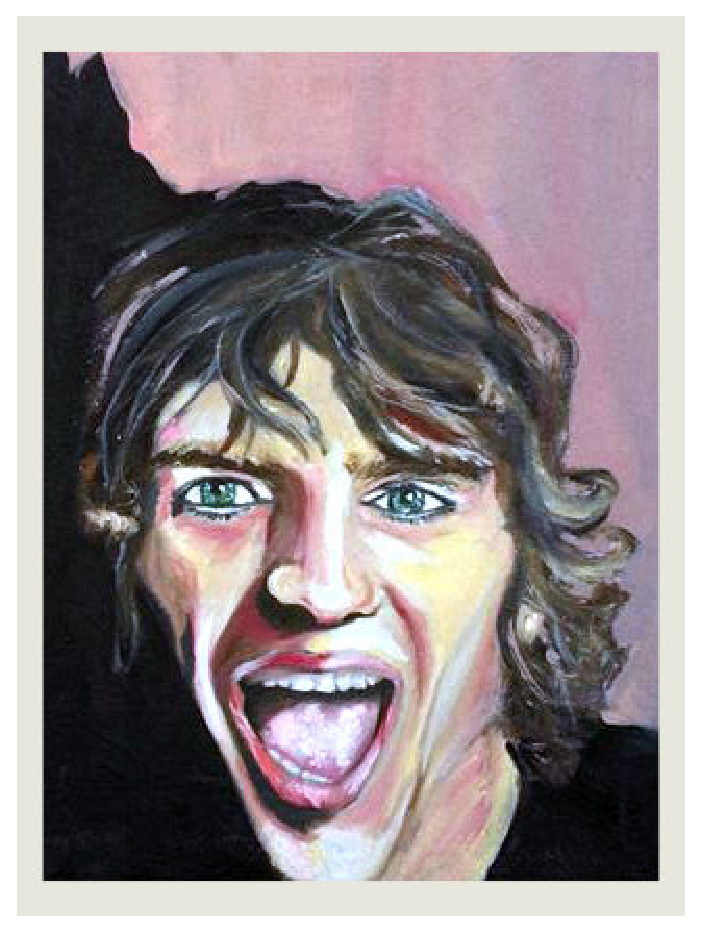
\includegraphics[scale=.50]{../eps/face.eps} 
\caption{ABSTRACT PORTITURE- UNTITELED}
\label{label}
\end{center}
\end{figure}

Abstract expressionism taught me to let go of the end result and focus on the movement of the paint and the way I felt. Hence this allowed me to be flexible in the way I created mandalas, as I let the materials dictate what was being created and I was not fixed on the end result. In this process I was able to focus on the detail whilst being playful and I felt free to make mistakes. Mandalas have always made sense to me, as they give me a sense of relief from my emotional content that builds within me and feels difficult to hold.

My former partner and I lived and worked in Australia for 9 years before moving to Cambodia for 3 years. I was working as an Arts Therapist and Counsellor, both in voluntary and paid positions, amongst other jobs to pay the bills in Cambodia. For two and a half years I worked with the Ragamuffin Project in Cambodia where we supported children and young people with multi complex traumas. I also worked with Indigo Psychological Services, where we worked with western clients; both were amazingly powerful and depressing. 

My work supervisor Carrie Herbert, encouraged me to look after myself by using experiential art mediums and keeping case notes brief and succinct. Having permission to create and attend to my self-care through using a medium that made complete sense emotionally, physically and psychologically was liberating, and intensified my passion for mandalas. I then started to use mandalas as a self-reflective and debriefing tool, along with supervision and writing case notes. I mostly kept a small sketch book of mandalas, as I regularly travelled a lot. Every second weekend I would catch a six-hour bus ride to the Province so I needed to pack light, as it was only for two nights. I also felt that minimising the actual size of the mandalas was important due to time factors that also helped to get to the essence of my experience for that session or day.
I yearned for further professional development and wanted to advance my qualifications whilst living in Cambodia. After returning to Australia with the mission of undertaking my masters. I noticed mandalas were always at the forefront of my awareness and I was conscious that there was something really important to explore and inquire into but I did not know why.

\section{Beginning my inquiry}

When I began my exploration, I was interested in the two following topics:
\begin{itemize}
\item mandalas, because I feel connected to the process. 
\end{itemize}

\begin{itemize}
\item emotions, mainly because I feel we are so out of touch most of the time. 
\end{itemize}

However, I quickly realized that emotions naturally are a part of the process of inquiring into creating a mandala. So essentially, I was inquiry into the two things that I held important to explore through my Masters process.  
My supervisor Dr Jan Allen suggested that I take a few different angles as I inquired into the process of creating mandalas.

\newpage

\begin{enumerate}
\item Drawing a mandala whilst tracking and writing all my thoughts, sensations, emotions and memories down 
\item Drawing a mandala and then dialoguing with it 
\item Drawing a mandala and then using MIECAT methods of inquiry to explore my understanding 
Initially, I mainly drew mandalas which tracked my emotions, thoughts, sensations and memories. I enjoyed slowing down all my thoughts and feelings, I became lost in the stillness at times and then took a breath back into the present feeling, memory and emotions. 
\end{enumerate}















	%Beginning my inquiry (section) 

%Background (chapter

\chapter{Background}
\begin{quote}
"Jung states a Man cannot stand a meaningless life" (C Jung) 
\end{quote}

\newpage
\begin{figure}[h!]
\begin{center}
\includegraphics[scale=.25]{../eps/In_through_the_background.eps}
\caption{In through the background}
\label{label}
\end{center}
\end{figure}

\newpage
Before I start my inquiry, I want to orient you the reader and provide a small window illustrating the complexity of what mandalas can pose and why I hold drawing mandalas so dear to my heart. 

I sat down to reflect on the mandalas I have kept over the years and one stood out for me. I sat with this mandala which I produced in 2005 and was astounded by the message it had for me 10 years after producing it and I still remain fascinated by what it might continue to teach me in the future. I continue to be curious in particular about the power of mandalas and what the symbols represents as well as what resonates for me now. 

I explored two mandalas which were created 10 years apart, but remarkably have a connection and seem to be unified.   

The following mandala I drew on the 22 of November 2005 (which was the third year out of the twelve years my former partner and I were together) I drew this mandala in response to a dream amplification: 

\begin{figure}[h!] 
\begin{center}
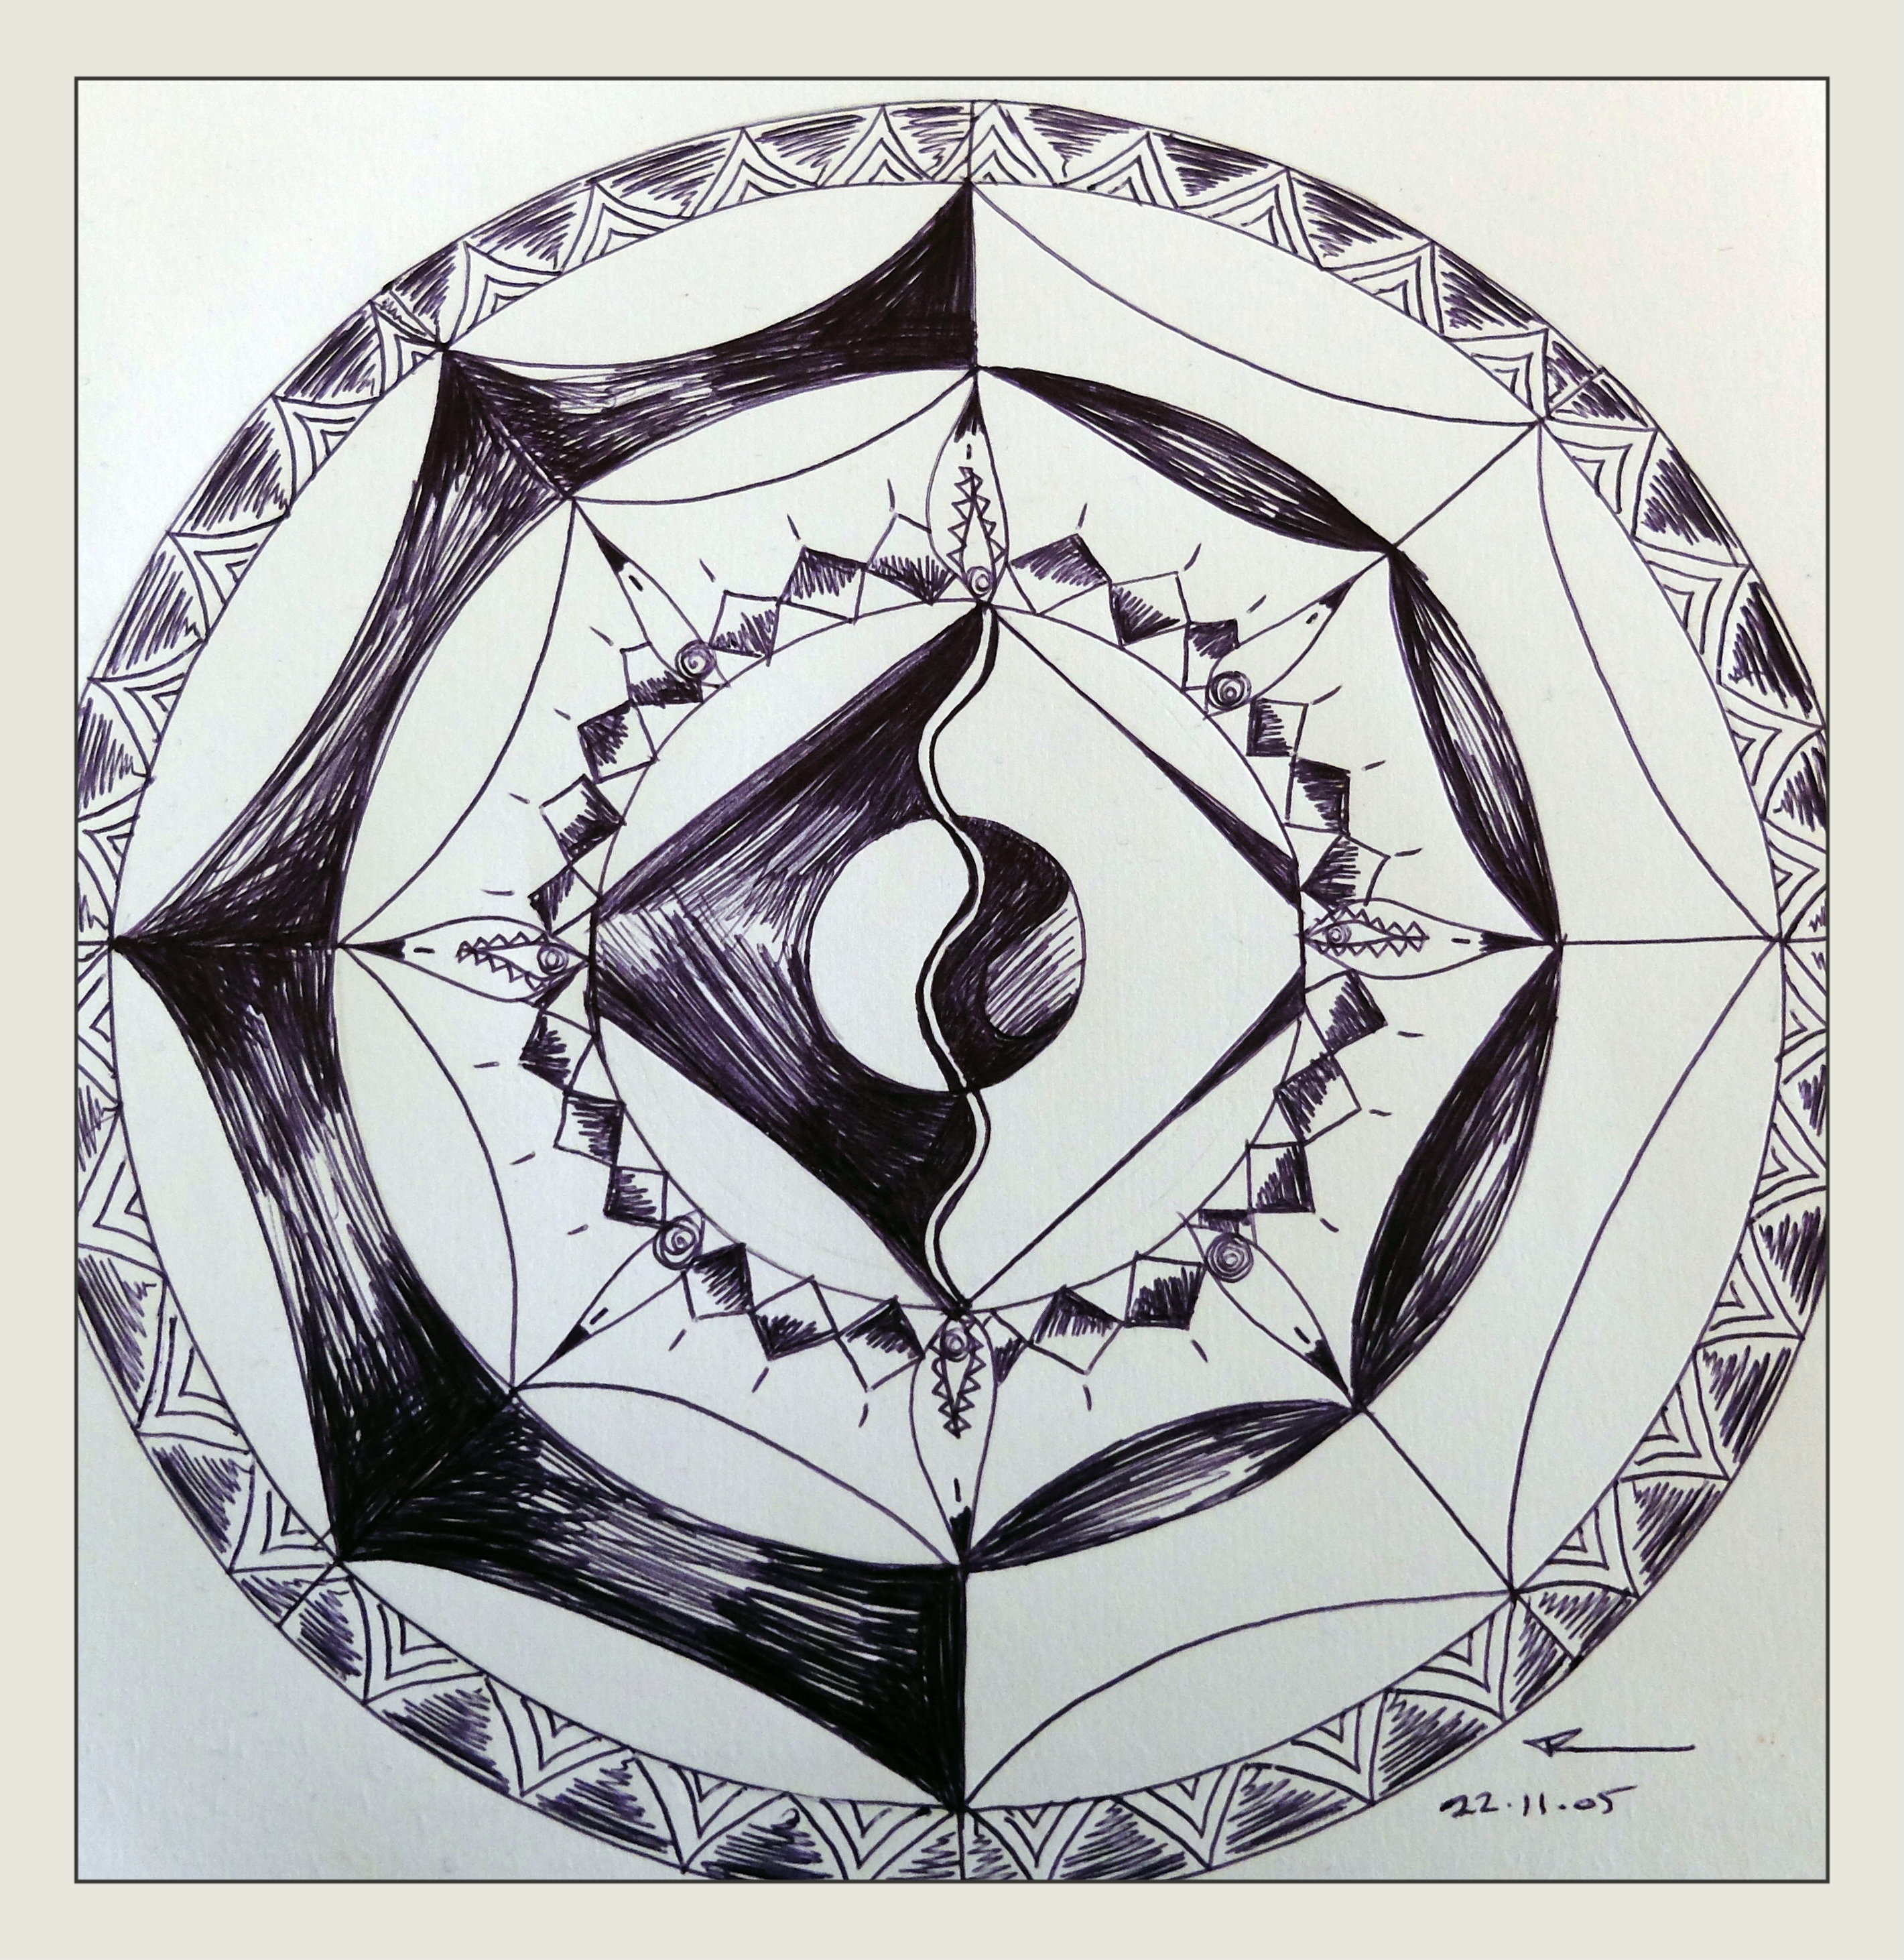
\includegraphics[scale=.1]{../eps/2005_m.eps}
\caption{2005 Mandala}
\label{label}
\end{center}
\end{figure}

%FIGURE 2-2005 MANDALA (try and get this up in this placement 

And wrote in my journal: \newline 

I have many dreams where we have broken up, as he has cheated on me, however I never thought he would actually cheat in real life. I feel that this dream is an indication of my fear of abandonment. We have been together for 3 years. He has never wanted to comment on our future which bothers me as it poses the question- When will he break up with me? Perhaps my ego is trying to balance my relationship and my emotions. I feel a lack of attention from him, not being able to ease my emotions about being together and not knowing when he might pull the rug from under me. I also feel my dream is also trying to communicate that I need to break away from a situation or any bad habits that I may have. As well as being balanced within myself and accept myself and stop with the self-deprivation.  

It is amazing that 10 years after I produced this mandala in 2005, my former partner did pull the rug from under me. He ended our relationship in 2014 abruptly without warning. He withdrew and disappeared to never say another word to me. I still remember how I felt in the dreams I had when he broke up with me. All those years later, when he did end our relationship, he behaved exactly like in my dreams. He was cold, empty, no compassion and had totally withdrawn. The only thing he revealed was that he felt lost and did not know what he wanted. I, on the other hand, had very clear goals; I wanted to complete my masters and to start a family with him. But after 12 years he was just as confused when I met him regarding what his aspirations were. I was attracted to his intelligence, his many talents and his beautiful blue eyes. He was my best friend and lover for 12 years and never spoke about being unhappy in our relationship, but at the same time he never commented on how he saw our future, even when we decided to get engaged in late 2013. 

Reflecting on the phrase of pulling the rug from under me, I have only now been able to understand the significance of this symbolic rug. It now makes perfect sense why I felt it was so important for me to keep the beautiful rug we bought in India. We did not have many possessions but the rug was the only thing that I yearned for when we went our separate ways. I felt lost when he left as it was excruciating and so sad that he chose to walk away and vanish. However, in my grief, I remained grounded and I never lost sight of who I was. Thus, it was invaluable for me to put my own feet on this beautiful soft rug and not get caught up in my self doubt around the questions why he left.


\begin{figure}[htbp]
\begin{center}
\includegraphics[scale=.2]{../eps/My_rug_.eps}
\caption{MY RUG!}
\label{label}
\end{center}
\end{figure}


Fast forward to the 8th of August 2015 to intensive three class for the MIECAT Masters program; after exploring my embodiment, I intuitively created a mandala which served as my new mantra. 



%FIGURE 4-MANDALA MANTRA
%FIGURE 5- DEFFINITION OF THE MANDALA MANTRA
%Get better picture and size

After my former partner revealed he wanted to separate, I woke up with the word reciprocity stuck in my head which has evidently stayed implanted in my body. As soon as I drew this wiggled line, I knew it represented reciprocity and balance for me. This wiggled line is similar to the shape of an 'S'. The wiggled shape is going through five different coloured circles, which are the same on either side of the wiggled line. They overlap each consecutive circle which is encompassed within a large circle. Each of these circles represent qualities I desire in an intimate relationship. 

They are as follows:
\begin{itemize}
\item Affection (white)
\end{itemize}

\begin{itemize}
\item Affirmation (red)
\end{itemize}

\begin{itemize}
\item Connection (green)
\end{itemize}

\begin{itemize}
\item Acknowledgment (yellow)
\end{itemize}

\begin{itemize}
\item and for the both of us to be Grounded (brown)
\end{itemize}

    
To my surprise this wiggled line is also similar to the centre of the mandala I drew all those years earlier in 2005, although in this early mandala this wiggled line is in the opposite direction. In the 2015 mandala the wiggled line has two different colours- red and green that slightly overlap each other in the centre of the line. In 2005 there is only black and white. This is quite interesting as in the past I looked at the world with a very black and white mentality but now I can see the world has so many more colours that blend into each other. It is refreshing to be able to appreciate their ever shifting elements and not be stuck in this fixed terminology. 



%FIGURE 6- 2015 MANDALA MANTRA
             		

%FIGURE 7- MANDALA 2005

Take a double exposure picture of these two mandalas



	%Background into my inquiry(section)

	
	%Methods and Methodology (chapter)
	
	
	
	\newpage
\chapter{Methods and Methodology}
\begin{quote}
"The power of an image is that it embodies the complexity of what we see, feel and think but cannot literally describe in words." Tufnell and Crickmay, p.(2004)
\end{quote}

\newpage

\begin{figure}[htbp]
\begin{center}
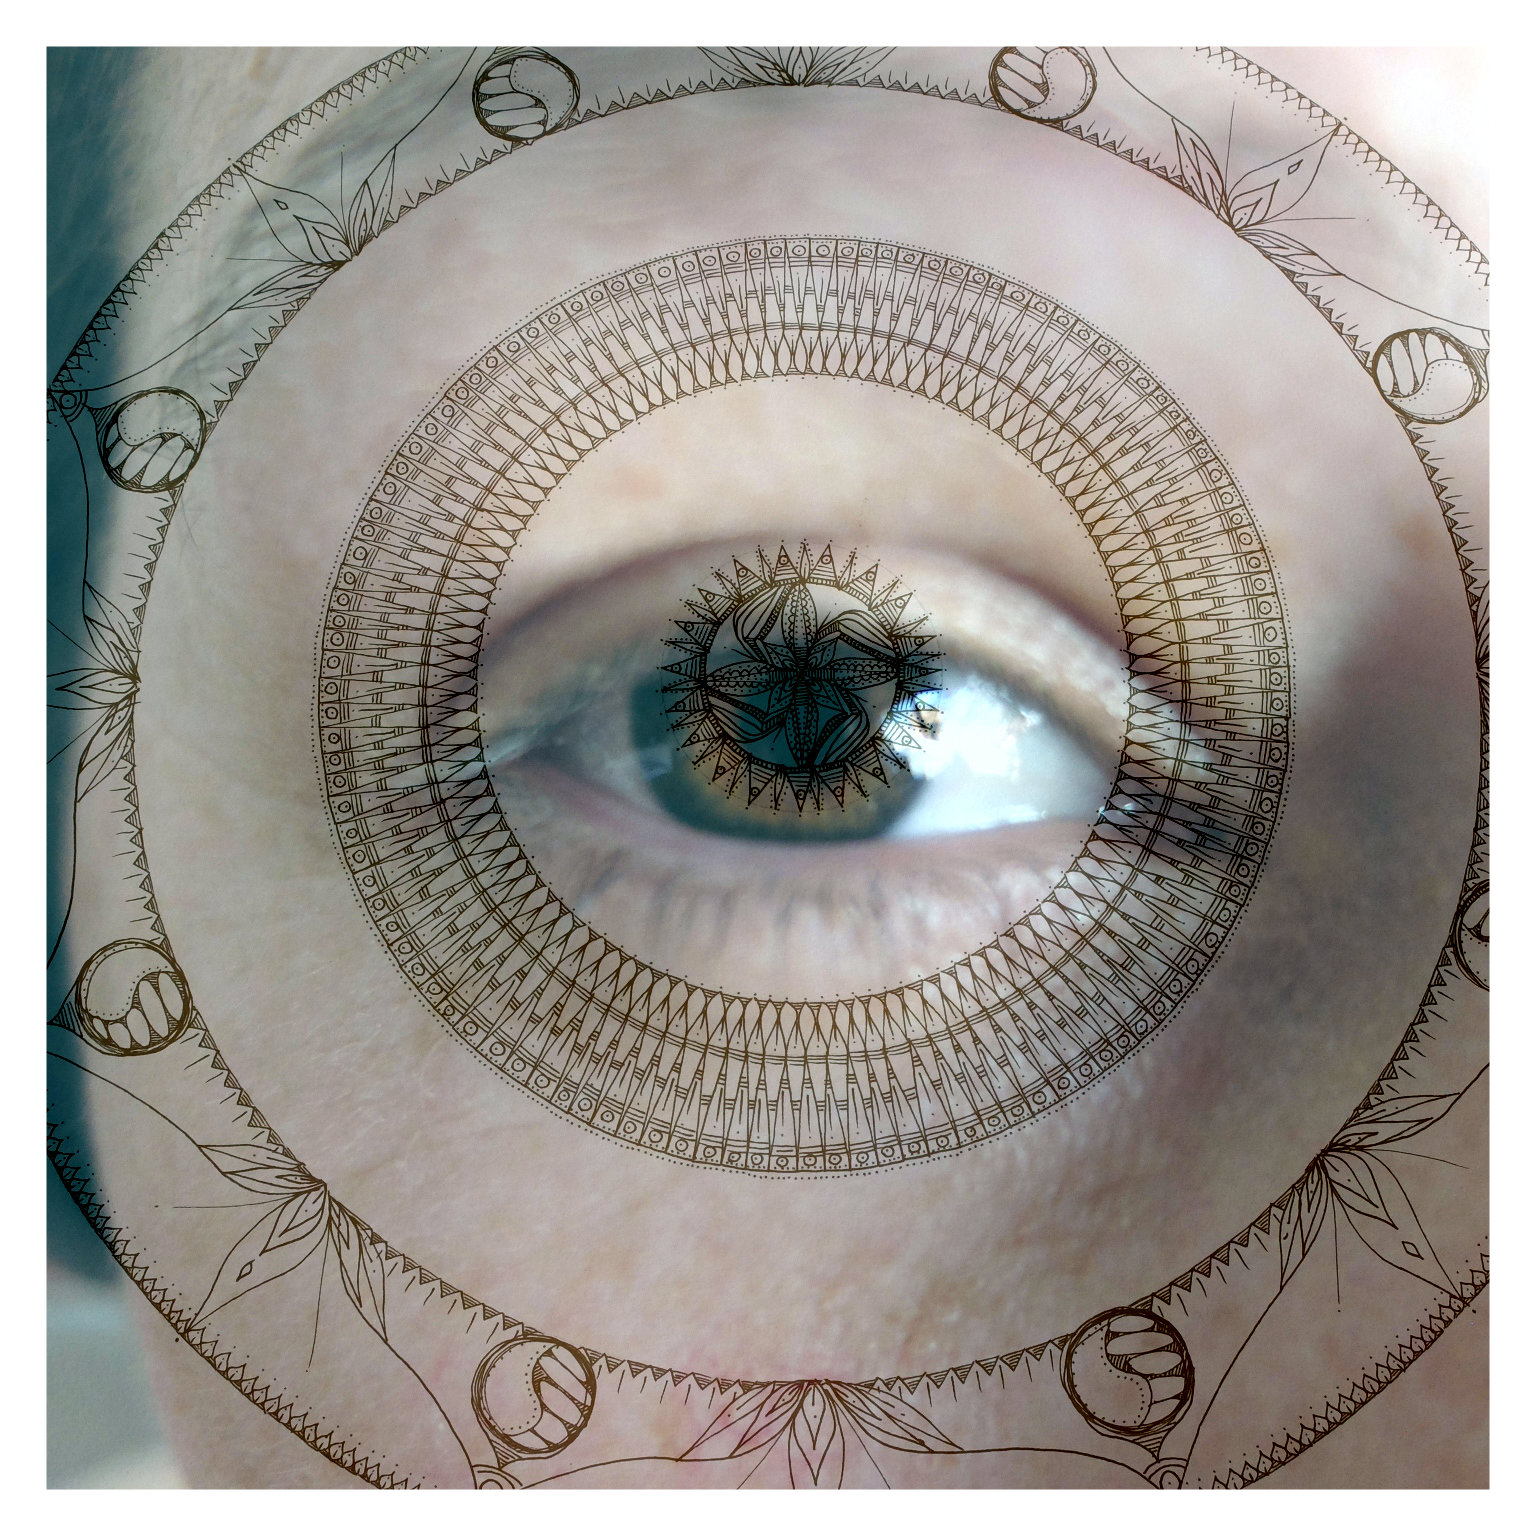
\includegraphics[scale=.3]{../eps/Double_exposure_eye_mandala.eps}
\caption{Double exposure eye mandala}
\label{label}
\end{center}
\end{figure}
%FIGURE 1-DOUBLE EXPOSURE WITH MY EYE AND MANDALA

\newpage

As you have already read, my research inquiry starts with my passion for drawing mandalas and I inquire into the journey of what I have come to know through this process. 
\begin{enumerate}
\item I began with an introduction and background information why I am inquiring in mandalas.  
\item I now move into my methods and methodology. As well as my procedures, paradigm alignment and my values I hold within my thesis. 
\item 
Following my methods and methodology I have predominately worked with my own data. I have drawn 6 mandalas and I have described the following: the making process of each mandala, key words, dialogue which happened within the process as well as pictures which illustrates the process of creations. You will find the following 6 mandalas in the following chapters. After the 6 mandalas, I have further explored and amplified them. 
\item 
Next, I have also included others experiences of drawing mandalas and their perspectives in my inquiry.
\item 
I then present the key words and essence words which are derived both my participants and from my own data. 
\item 
Then, by focusing on the process of drawing a mandala within a therapeutic context and its relevance and benefits. I provide with a creative synthesis and practical example to conclude.
Update 
\end{enumerate}

\section{Methodology}

My research is qualitative and circular. The notion that a circle has no beginning nor end is similar to the concept of us continuously evolving, shifting and transforming as beings. Throughout my process of drawing within mandalas I have continuously shifted and evolved within myself. 

I consider mandalas to have the capacity to delve into my unconscious parts of myself and cut through any pretence. Words do not come naturally for me, but images do. When I use my imaginative visualizations and images I create, I step beyond my analytical restrictions and become liberated to bring together my vocabulary and imagery and thus make sense of the experience I am exploring. Consequently, when attending to these key images, I feel they connect me with my pre-reflexive knowing and help to form my new knowing. 

The word mandala comes from the Sanskrit word which denotes essence and circle. Mandalas are ancient and have been used throughout history within many different cultures and religions. Thus, indigenous cultures used mandalas as symbols for healing and transformation. However, research into the healing aspects of drawing mandalas in the psychology field are rare. 

\section{Methods}


I have chosen an Arts as Inquiry approach which uses the arts first-hand in the inquiry to conduct meaning making from the arts itself. This inquiry uses many different modalities such as: drawing, movement, photography, sound, play, poetry and tattooing.

I have also used The MIECAT form of Inquiry, which has no predetermined or fixed methodology. Instead the process allows an emergent integrative flow of knowing and ways of being in the companioning process.  

The MIECAT form of Inquiry strengthens the feeling-emotion-thinking-valuing connectedness and attends to the here and now with a subjective and descriptive manner. The inquiry is placed around making meaning of the lived experience and what we have come to know. Dr Dan Siegel states: 

\begin{quotation}
"We need to empower people and say it is not what happened to you, it is how you make sense of what happened to you. He also said that the research also shows, that you are likely to repeat that, wether it's abuse, neglect or emotional distance if you have not made sense of those experiences." 
\end{quotation}

As Lett says 
\begin{quote}"since so much experience is not encoded verbally, and the explication of stored meanings is usually more complex than verbal skills alone can convey." (p, 1992) 
\end{quote}

When we combine multimodalities with dialoguing and experiencing pre-reflective and less conscious states, we bring together a variety of languages of the visual nature, pre-reflective knowings and intuition in combination with our cognitive language. Thus, by using a variety of modes we gain access to our own wisdoms, as well as having a better understanding of ourselves and the world around us. 

The procedure I used in my quite conversations within mandalas was an Arts as Inquiry. I was open to the awareness of my body and I endeavoured to stay present to my felt sensing. I bracketed in and out my thoughts. I also had a sense of moving in and out of collapsed time. In this collapsed time, I embark into my memories and simultaneously experienced the feelings of the present and the past. 

Hypnotically, I move the piece of paper around whilst I draw. I drift away with my emotions and feelings and at times my thoughts were in a vacuum of nothingness. I simply draw the same line over and over and, as a result, I become so immersed in the drawing process that I forgot to write key words as I had initially intended. 

Creating a mandala, I start by drawing a large circle with the compass, then keeping the sharp end in the paper, I move the pencil end of the compass, to make a few more circles within the larger circle.  I work from inside out and I intuitively make lines, dots and shapes. I never use measurements or sketch out the design. As McNiff says:
\begin{quote} "I can never know in advance what will appear, because I discover what is going on inside me through the process of painting." (p,1998). 
\end{quote}

I feel that any process of creativity is the same when it comes to discovering what is inside us. The only element in my mandalas which is not drawn freehand is the circles drawn with a pencils on the compass. These circles are erased and function as lines on the page to guide me.  


\section{Procedures}


\begin{figure}[htbp]
\begin{center}
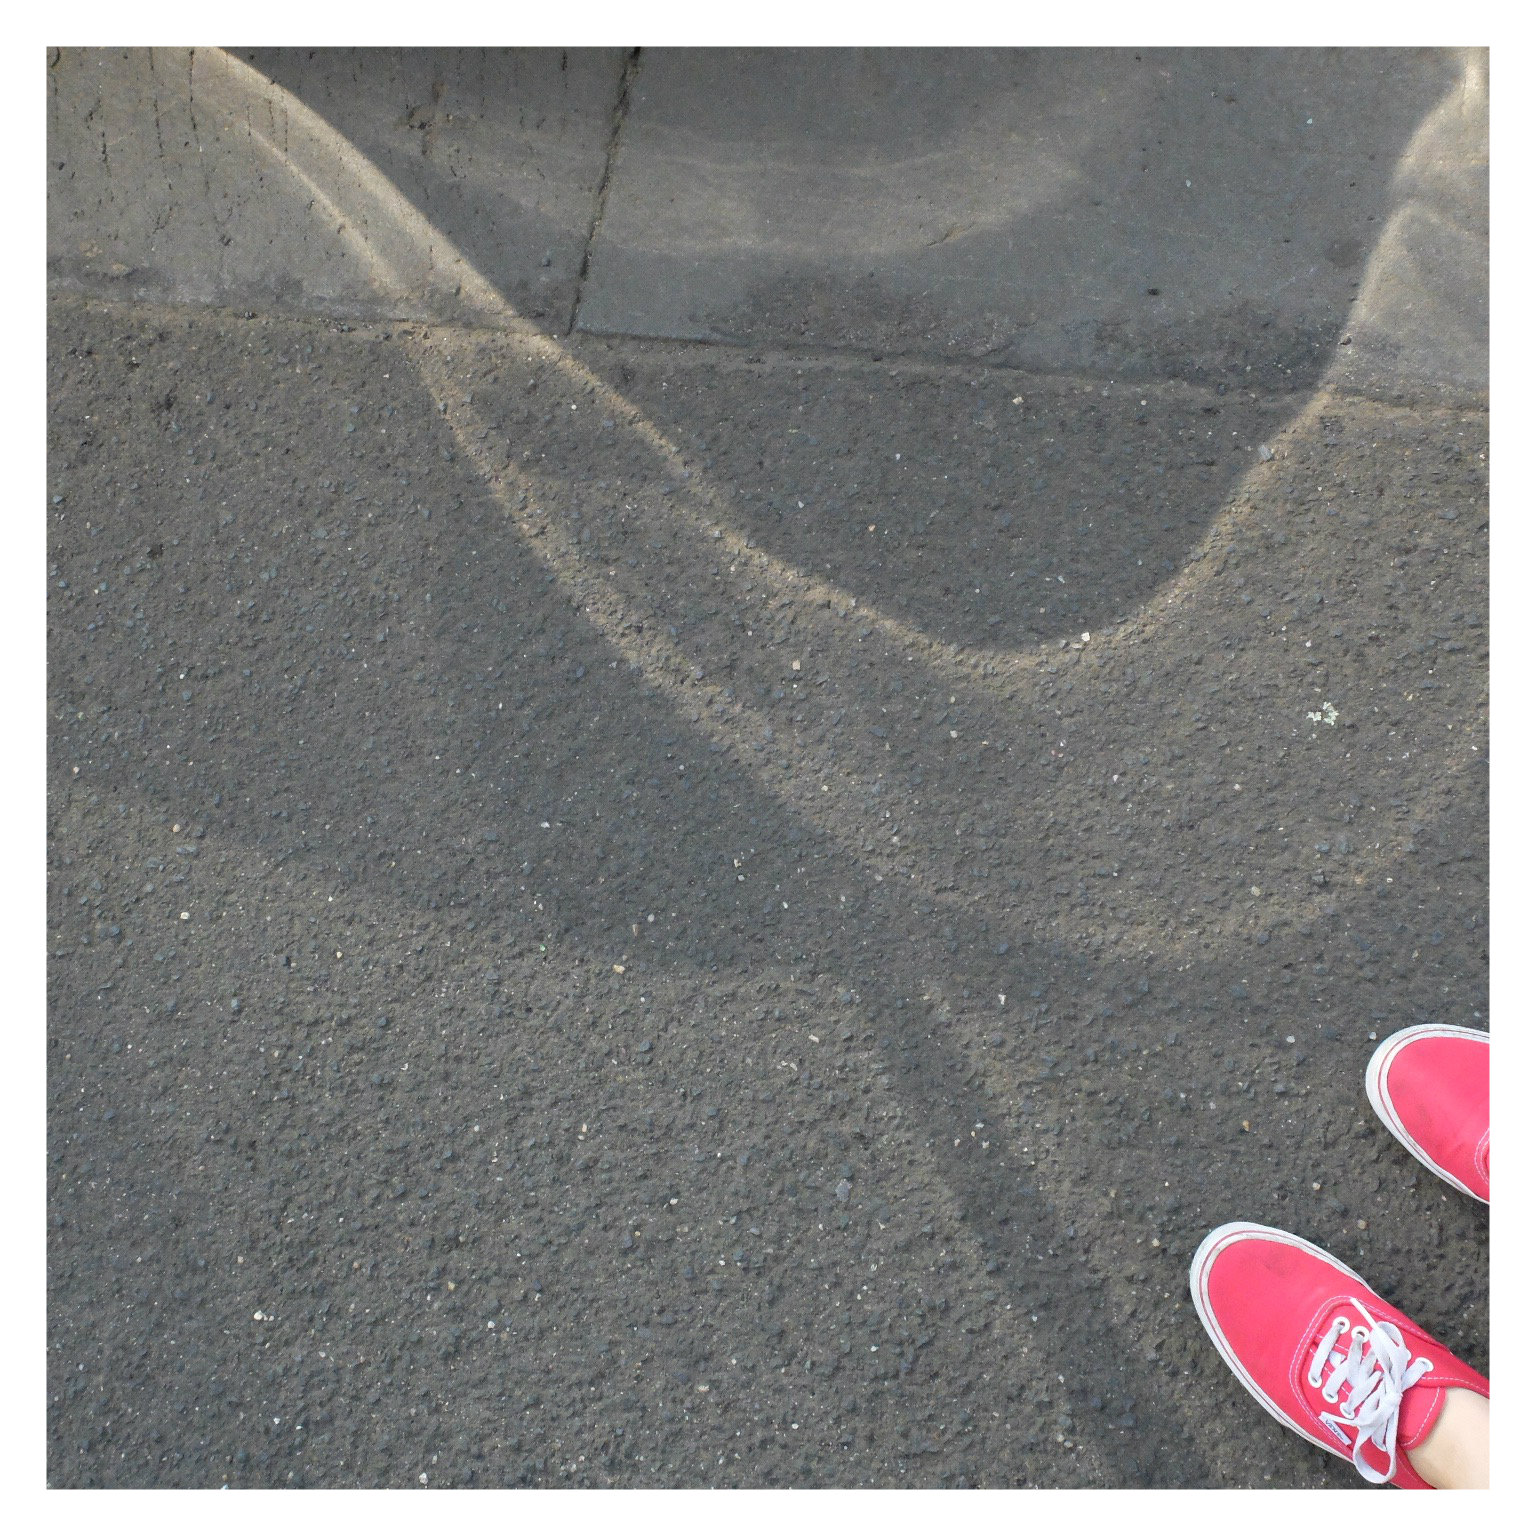
\includegraphics[scale=.3]{../eps/Stepping_into.eps} 
\caption{The procedures I stepped into}
\label{label}
\end{center}
\end{figure}

%FIGURE 2-THE PROCEDURES I STEPPED INTO


The procedures I used in creating and making my own mandalas are the following:
\begin{itemize}
\item Attending to the present moment
\end{itemize}

\begin{itemize}
\item Accessing lived experiencing 
\end{itemize}

\begin{itemize}
\item Finding emergent expression through mandala form
\end{itemize}

\begin{itemize}
\item Starting off with my emotional state, engaging with art making and noticing the changes and shifts within myself
\end{itemize}

\begin{itemize}
\item Remained with a descriptive attitude 
\end{itemize}

\begin{itemize}
\item Key words
\end{itemize}


After drawing the 6 mandalas, I remained attuned and aware to the slightest changes within me. I sat with all my personal data to deliberately amplify its content to come up with the themes and topics which arose. I also kept generating more data as the year went on through keeping a mandala diary. 
Additionally, I added these procedures to the mix: 

\begin{itemize}
\item Reduction to what is important 
\end{itemize}

\begin{itemize}
\item Essence key words/images
\end{itemize}

\begin{itemize}
\item Clustering key words
\end{itemize}

\begin{itemize}
\item Designing and getting a tattoo
\end{itemize}

\begin{itemize}
\item  'I' poems- An 'I'poem is the process where a piece of text is underlined only with the I and the accompanying word. This highlights associative stream of consciousness carried by the first person and how the writer speaks about themselves. (Gilligan, spencer, Weinberg, Bertsch 2006). On the listening guide- A voice-centred relational methods, Gilligan, spencer, Weinberg, Bertsch 2006, Sage publications
\end{itemize}

Within the process of my own work and companioning others, the following procedures are adapted to the context and situations. They are as follows:
\begin{itemize}
\item Description- where one is descriptive and states what can be seen in basic terms 
\end{itemize}

\begin{itemize}
\item ISR- (Intersubjective response)- a response offered to the other
\end{itemize}

\begin{itemize}
\item  Clustering- grouping together images and words which fit together* Representations- can be expressed through using many art modality art forms
\end{itemize}

\begin{itemize}
\item Reduction- reducing large images and text to key words and images 
\end{itemize}

\begin{itemize}
\item Bracketing- where we bracket in and out our own thoughts, as well as being aware of our own feelings and sensations only sharing with the other what is helpful and appropriate
\end{itemize}

\begin{itemize}
\item Accessing to experiencing- We can sense or be aware of our less conscious states along with conscious parts through accessing our experiences through connecting to our emotions, thoughts, sensations, imagery, memories, smell, visualisations, bodily sensations and feelings
\end{itemize}

\section {Maps}
The following are mind maps of the steps and procedures I took:
%maps



\section{Paradigm alignment}

\begin{figure}[htbp]
\begin{center}
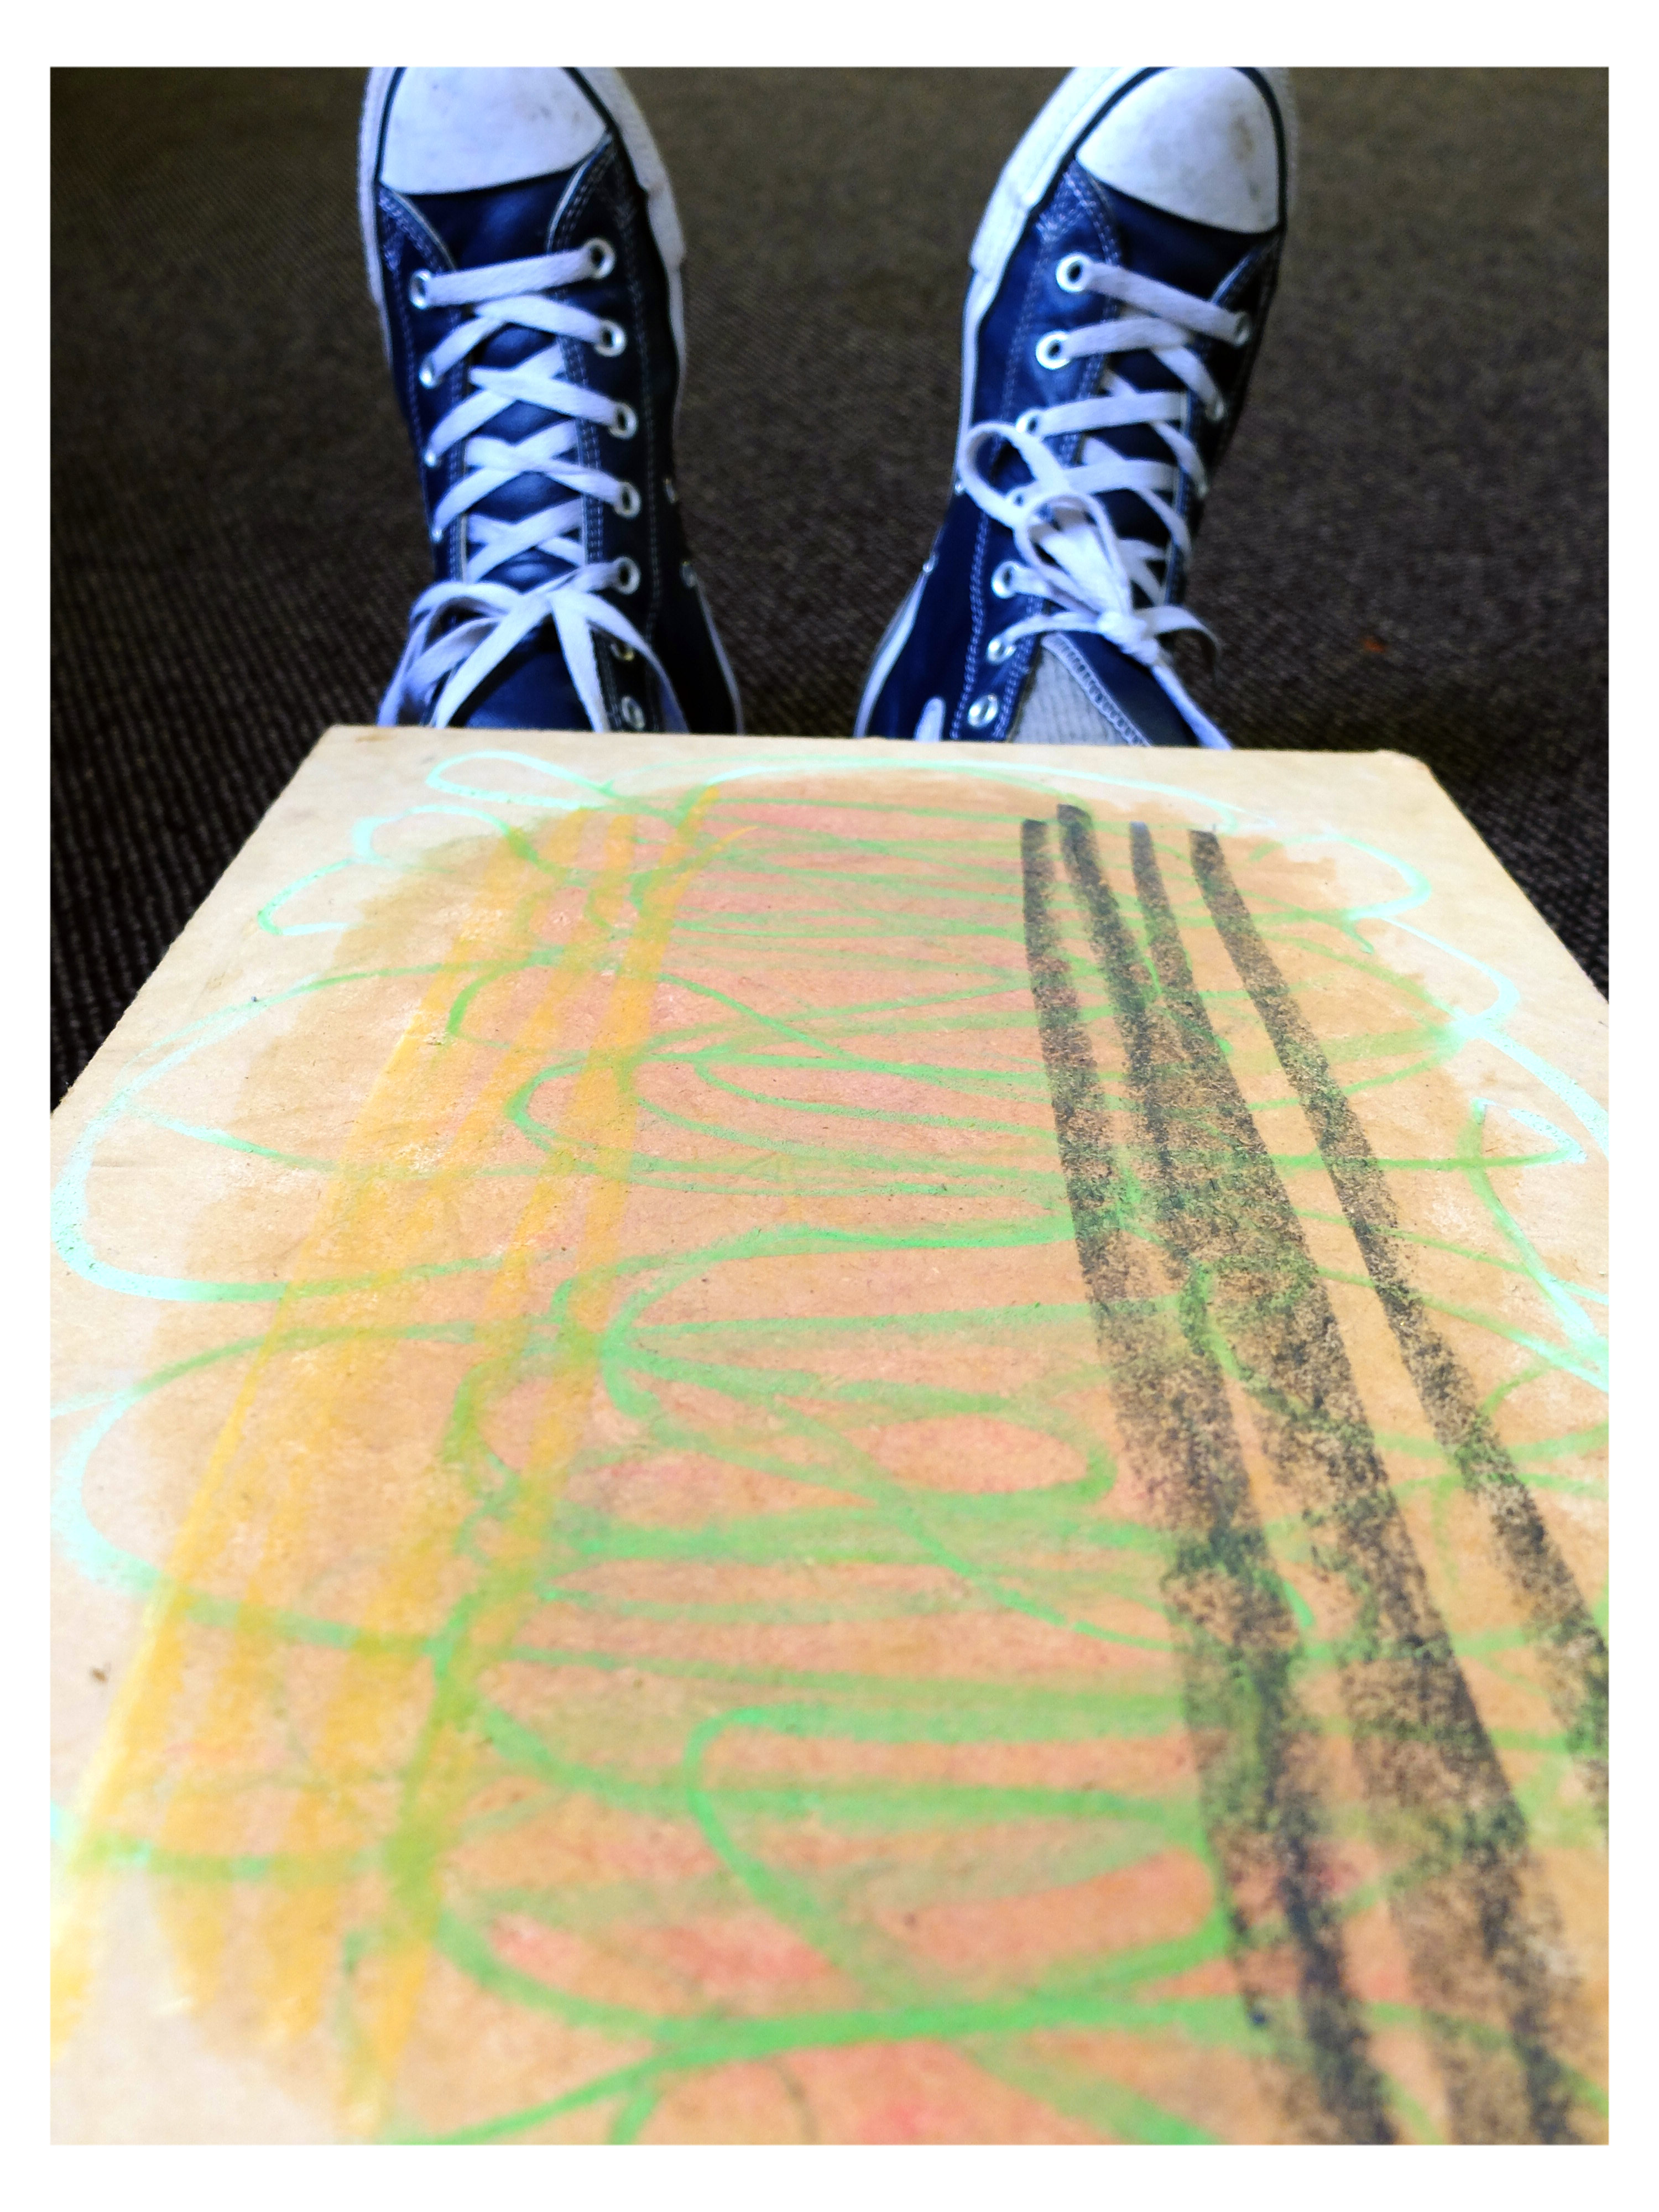
\includegraphics[scale=.1]{../eps/My_allignment_and_shoes.eps} 
\caption{My alignment and shoes}
\label{label}
\end{center}
\end{figure}
\newpage

%FIGURE 3- MY ALIGNMENT AND SHOES


Things are not as fixed as I once thought, hence I have come to know that I sit in a Post-modern paradigm. We are relational beings and we constantly change and evolve. We are in an integrative flow and companion and co-construct every moment. Therefore, we all make the choice to participate and inquire into each other and our relationships around us. I feel we need to take the time to re-connect both with others and ourselves because of this constant evolution of our lives. I wrote this in reflection:


\begin {centering}As they change, we change\newline 
As we change, they change\newline 
So, do we accept or do we fight it?\newline 
Do we ignore it or adapt?\newline 
Is it hidden or do we see it?\newline 
We aspire to relate and connect\newline 
And as we change and they change\newline 
We make the choice\newline 
To transform together or apart\newline 
\end {centering} 



\begin{figure}[htbp]
\begin{center}
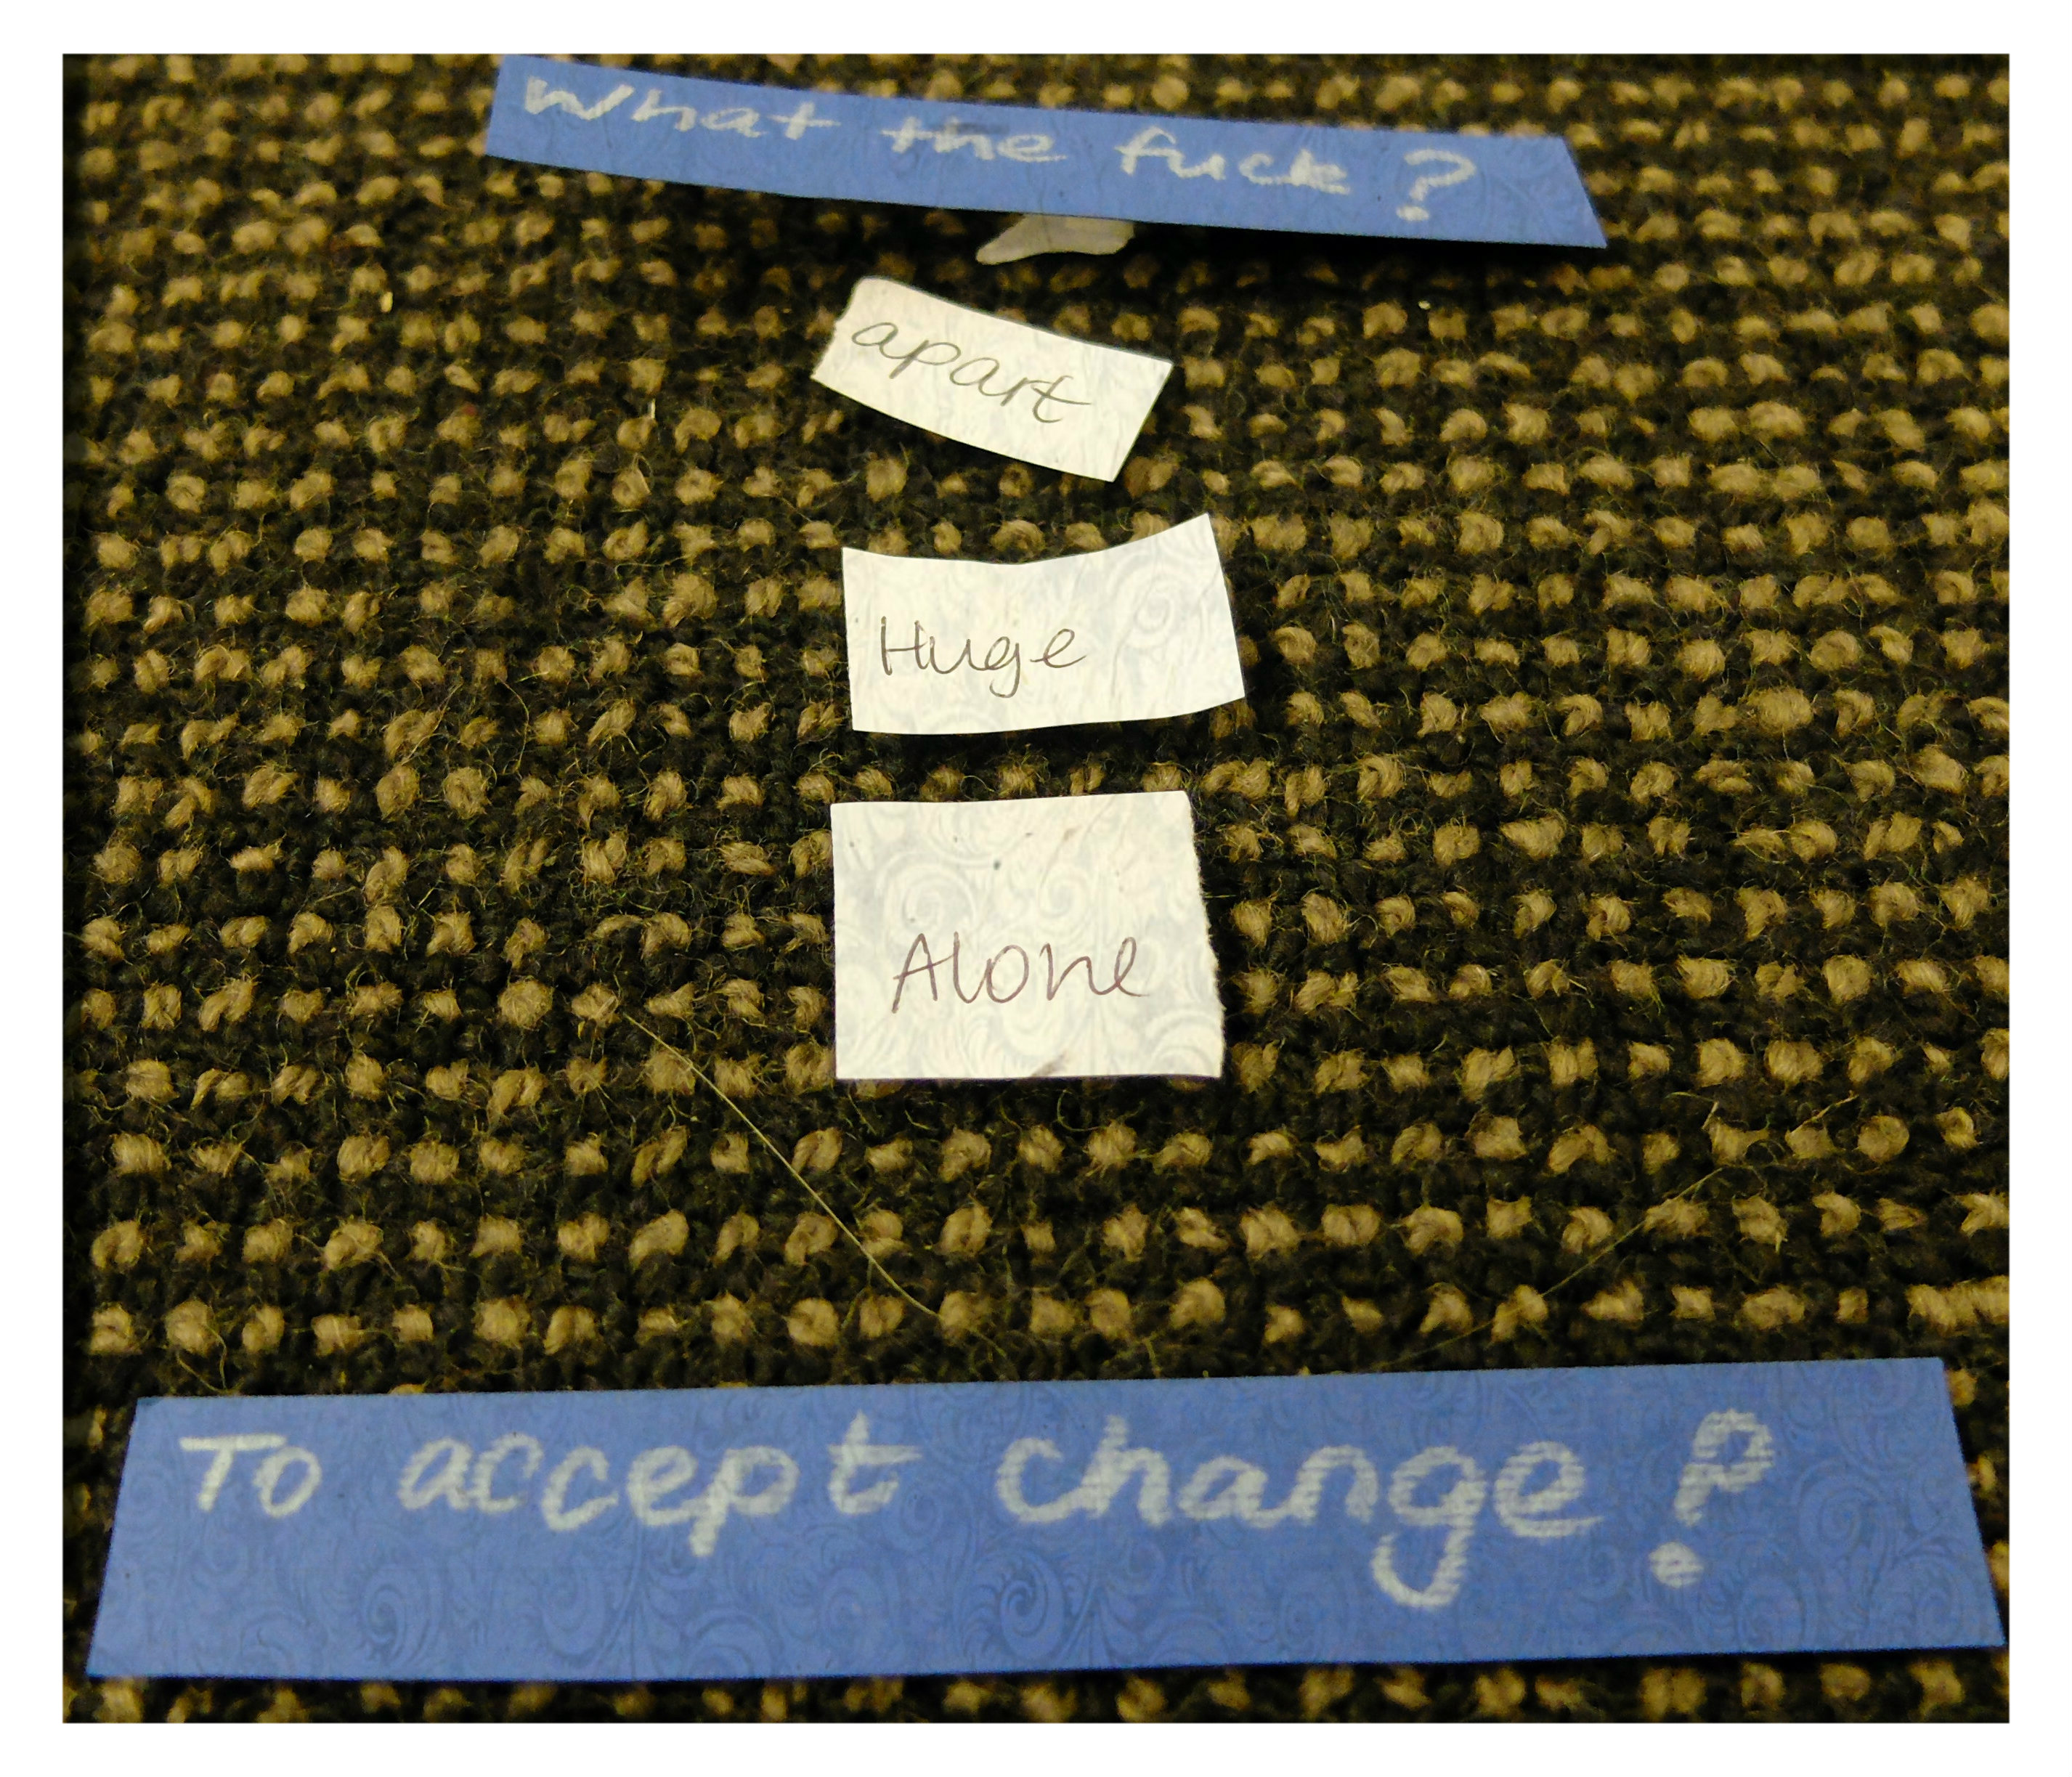
\includegraphics[scale=.1]{../eps/What_the_fuck.eps} 
\caption{What the fuck?}
\label{label}
\end{center}
\end{figure}
\newpage
%FIGURE 4- WHAT THE FUCK?




	
	
	
	%Methodology (section)
	%Methods (section)
	%Procedures (section)
	%Maps (section) 
	%Paradigm alignment (section}
	
%Values (chapter)
	%Connection
	%Clarity
	%Imaginative visualisation 
	%Emergence

%Mandala 1
%Mandala 2
%Mandala 3
%Mandala 4
%Mandala 5
%Mandala 6

%Amplification of clusters

%Incorporating my participants into my inquiry

%My findings (chapter) 
	%section 1
		%setting the scene
	%section 2
		%The making of an embodied mandala 
	%Section 3
		%The emergence and re-looking process of a mandala
	%section 4
		%Broader application
	%section 5
		%practical example of self care
		%My tattoo sybthesis
		%tattoo process


\end{document}


